\begin{frame}{Features}
\centering
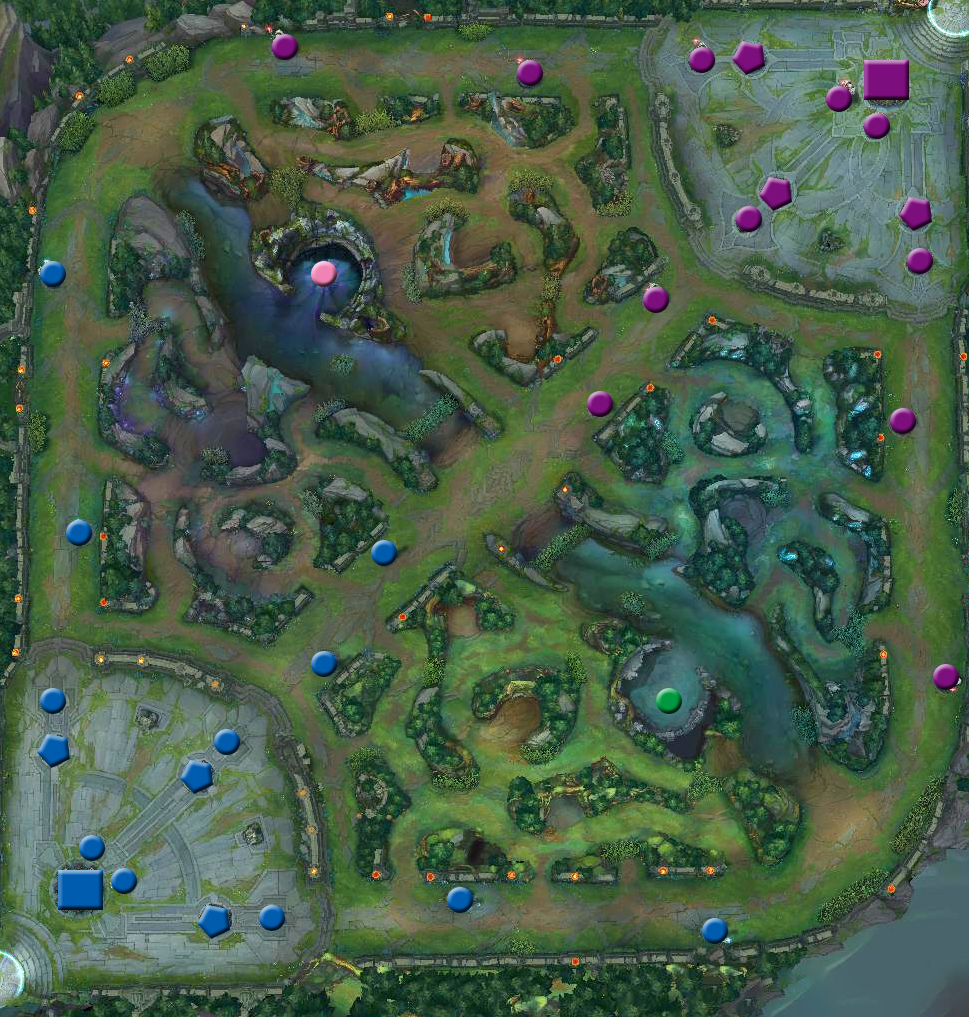
\includegraphics[scale=0.2]{img/kent/lolmap.jpg}
\end{frame}

\begin{frame}{Features}
\centering
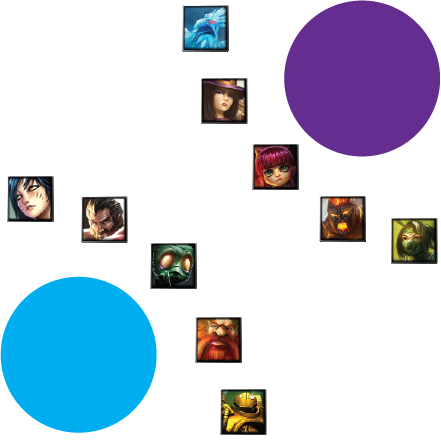
\includegraphics[scale=0.35]{img/kent/1.png}\\
\vspace{8pt}
$P(Winner = \textcolor{blue}{\text{blue}}) = \alpha$
\end{frame}

\begin{frame}{Features}
\centering
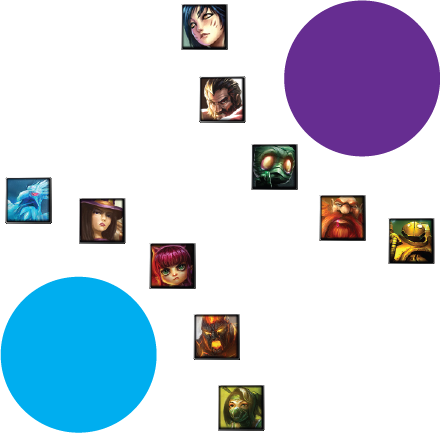
\includegraphics[scale=0.35]{img/kent/2.png}\\
\vspace{8pt}
$P(Winner = \textcolor{purple}{\text{purple}}) = \alpha ?$
\end{frame}

\begin{frame}{Features}
\centering
\textcolor{blue}{Team blue} (won)

\includegraphics[scale=0.4]{img/kent/pickblue.png}\\
\vspace{20pt}
\textcolor{purple}{Team purple} (lost)

\includegraphics[scale=0.4]{img/kent/pickpurple.png}\\
\end{frame}

\begin{frame}{Binary representation}
\centering
\textcolor{blue}{Team blue} (won) \hspace{40pt} \textcolor{purple}{Team purple} (lost)\\

\includegraphics[width=0.47\textwidth]{img/kent/pickblue.png}\hspace{2pt}%

\includegraphics[width=0.47\textwidth]{img/kent/pickpurple.png}\\
\vspace{18pt}
$\phi =$\\
\hspace{2pt} $(\textcolor{blue}{0,\;1,\;0,\;0,\;1,\;1,\;0,\;1,\;1,\;0,\;...},\textcolor{purple}{1,\;0,\;1,\;1,\;1,\;0,\;0,\;0,\;1,\;0,...})$\\
\vspace{18pt}
$y = \textcolor{blue}{\text{true}}$
\end{frame}

\begin{frame}{Mirrored binary representation}
\centering
\textcolor{blue}{Team blue} (won) \hspace{40pt} \textcolor{purple}{Team purple} (lost)\\

\includegraphics[width=0.47\textwidth]{img/kent/pickblue.png}\hspace{2pt}%

\includegraphics[width=0.47\textwidth]{img/kent/pickpurple.png}\\
\vspace{18pt}
$\phi =$\\
\hspace{2pt} $(\textcolor{blue}{0,\;1,\;0,\;0,\;1,\;1,\;0,\;1,\;1,\;0,\;...},\textcolor{purple}{1,\;0,\;1,\;1,\;1,\;0,\;0,\;0,\;1,\;0,...})$\\
$y = \textcolor{blue}{\text{true}}$\\
\vspace{18pt}
$\phi' =$\\
\hspace{2pt} $(\textcolor{purple}{1,\;0,\;1,\;1,\;1,\;0,\;0,\;0,\;1,\;0,...},\textcolor{blue}{0,\;1,\;0,\;0,\;1,\;1,\;0,\;1,\;1,\;0,\;...})$\\
$y' = \textcolor{purple}{\text{false}}$
\end{frame}

\begin{frame}{Compact binary representation}
\centering
\textcolor{blue}{Team blue} (won):\\
\hspace{20pt}
\includegraphics[width=0.47\textwidth]{img/kent/pickblue.png}\\
\vspace{8pt}
$\phi = (\textcolor{blue}{0,\;1,\;0,\;0,\;1,\;1,\;0,\;1,\;1,\;0,\;...})$\\
$y = \textcolor{blue}{\text{true}}$\\
\vspace{40pt}
\textcolor{purple}{Team purple} (lost):\\
\hspace{20pt}
\includegraphics[width=0.47\textwidth]{img/kent/pickpurple.png}\\
\vspace{8pt}
$\phi' = (\textcolor{purple}{1,\;0,\;1,\;1,\;1,\;0,\;0,\;0,\;1,\;0,\;...})$\\
$y' = \textcolor{purple}{\text{false}}$
\end{frame}

\begin{frame}{Ternary representation}
\centering
\textcolor{blue}{Team blue} (won)\\
\hspace{20pt}
\includegraphics[scale=0.31]{img/kent/pickblue.png}\\
\vspace{20pt}
\textcolor{purple}{Team purple} (lost)\\
\hspace{20pt}
\includegraphics[scale=0.31]{img/kent/pickpurple.png}\\
\vspace{20pt}
$\phi = (\textcolor{purple}{-1},\;\textcolor{blue}{1},\,\textcolor{purple}{-1},\textcolor{purple}{-1},\;0,\;\,\textcolor{blue}{1},\;\;0,\;\,\,\textcolor{blue}{1},\;\;0,\;\;0,\;\,...)$\\
$y = \textcolor{blue}{\text{true}}$\\
\end{frame}

\begin{frame}{Features}
\centering
\begin{figure}[!htb]
  \centering
  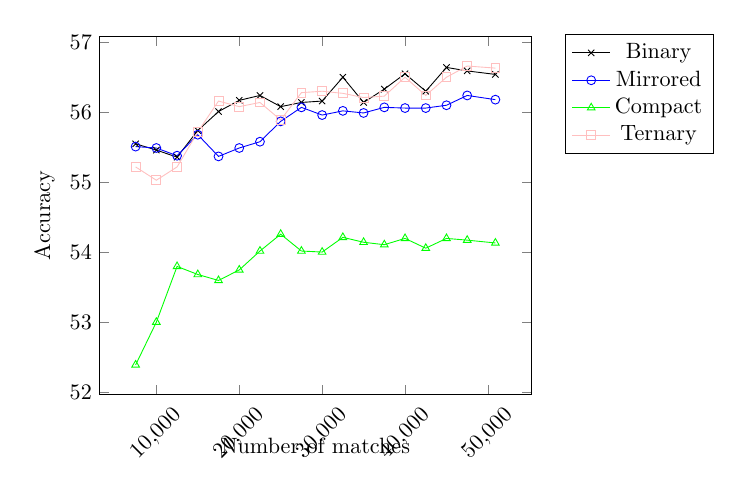
\begin{tikzpicture}[scale=0.8] 
    \begin{axis}[
      xlabel=Number of matches, 
      ylabel=Accuracy,
      xtick={10000,20000,30000,40000,50000},
      xticklabel style={rotate=45,anchor=near xticklabel},
      scaled x ticks=false,
      x label style={at={(axis description cs:0.5,-0.1)},anchor=north},
      legend style={at={(1.25,1.005)},
        anchor=north,legend columns=1},] 
      \addplot[color=black,mark=x] coordinates { 
        (7500, 55.55)
        (10000, 55.46)
        (12500, 55.36)
        (15000, 55.74)
        (17500, 56.01)
        (20000, 56.17)
        (22500, 56.24)
        (25000, 56.08)
        (27500, 56.14)
        (30000, 56.16)
        (32500, 56.50)
        (35000, 56.14)
        (37500, 56.33)
        (40000, 56.55)
        (42500, 56.30)
        (45000, 56.64)
        (47500, 56.59)
        (50901, 56.54)
      };
      \addplot[color=blue,mark=o] coordinates { 
        (7500, 55.51)  
        (10000, 55.49)
        (12500, 55.38)
        (15000, 55.68)
        (17500, 55.37)
        (20000, 55.49)
        (22500, 55.58)
        (25000, 55.87)
        (27500, 56.07)
        (30000, 55.96)
        (32500, 56.02)
        (35000, 55.99)
        (37500, 56.07)
        (40000, 56.06)
        (42500, 56.06)
        (45000, 56.10)
        (47500, 56.24)
        (50901, 56.18)
      };
      \addplot[color=green,mark=triangle] coordinates { 
        (7500, 52.395)  
        (10000, 53.005)
        (12500, 53.80)
        (15000, 53.685)
        (17500, 53.60)
        (20000, 53.75)
        (22500, 54.02)
        (25000, 54.26)
        (27500, 54.02)
        (30000, 54.005)
        (32500, 54.215)
        (35000, 54.145)
        (37500, 54.11)
        (40000, 54.20)
        (42500, 54.06)
        (45000, 54.20)
        (47500, 54.175)
        (50901, 54.135)
      };
      \addplot[color=pink,mark=square] coordinates {
        (7500, 55.22)  
        (10000, 55.03)
        (12500, 55.22)
        (15000, 55.72)
        (17500, 56.16)
        (20000, 56.08)
        (22500, 56.14)
        (25000, 55.89)
        (27500, 56.28)
        (30000, 56.30)
        (32500, 56.27)
        (35000, 56.21)
        (37500, 56.23)        
        (40000, 56.50)
        (42500, 56.24)
        (45000, 56.50)
        (47500, 56.66)
        (50901, 56.63)
      };
      \legend{Binary, Mirrored, Compact, Ternary}
    \end{axis} 
  \end{tikzpicture}
\end{figure}
\end{frame}

\begin{frame}{Features}
\centering
10 different types of features:\\
\begin{itemize}
\item Single champions
\item Pairs of champions
\item Champion counters
\item Player ranks (captured in 3 different ways)
\item Champion lanes
\item Champion spells
\item Champion runes
\item Champion masteries
\end{itemize}
\end{frame}


\begin{frame}{Features}
\centering
FeatureCreator:
\begin{itemize}
\item Introducing new features
\item Combining features
\end{itemize}
\end{frame}

\begin{frame}{Features}
Introducing a new type of feature:
\begin{itemize}
\item Initialiser function: Provide a unique name for all features
\item Feature extractor function: Given a game object, identify the features present in that game
\end{itemize}
\end{frame}

\begin{frame}{Features}
Introducing feature $\phi_\text{SINGLE,t,c}$
\begin{itemize}
\item Initialiser function: 
	\begin{itemize}
	\item $\text{BLUE-Ahri}$
	\item $\text{BLUE-Akali}$
	\item ...
	\item $\text{BLUE-Zyra}$
	\item $\text{PURPLE-Akali}$
	\item $\text{PURPLE-Ahri}$
	\item ...
	\item $\text{PURPLE-Zyra}$
	\end{itemize}
\item Feature extractor function:  
	\begin{itemize}
	\item Game object $\rightarrow \{\text{BLUE-Olaf}, \text{BLUE-Ryze}, \text{PURPLE-Lulu}, ...\}$
	\end{itemize}
\end{itemize}
\end{frame}

\begin{frame}{Features}
Introducing feature $\phi_\text{SINGLE,t,c}$
\begin{itemize}
\item Initialiser function:
	\begin{itemize}
	\item $\text{BLUE-Ahri} \rightarrow 1$
	\item $\text{BLUE-Akali} \rightarrow 2$
	\item ...
	\item $\text{BLUE-Zyra} \rightarrow 124$
	\item $\text{PURPLE-Akali} \rightarrow 125$
	\item $\text{PURPLE-Ahri} \rightarrow 126$
	\item ...
	\item $\text{PURPLE-Zyra}\rightarrow 248$
	\end{itemize}
\item Feature extractor function:  
	\begin{itemize}
	\item Game object $\rightarrow \{87, 96, 168, ...\}$
	\end{itemize}
\end{itemize}
\end{frame}